\documentclass[11pt]{article}

\usepackage{acl}
\usepackage{times}
\usepackage{latexsym}
\usepackage{amsmath}
\usepackage{multirow}
\usepackage{booktabs}
\usepackage{graphicx}
\usepackage{xcolor}
\usepackage{float}

\title{Multimodal and Agentic RAG for Grade 10 Mathematics Tutoring in the Nepalese Curriculum}

\author{
Nabin Lama, Anushka Ojha, Anubhav Kharel, Anish Kayastha \\
Asian Institute of Technology, Thailand \\
\texttt{st125985, st126222, st125999, st125988}
}

\begin{document}
\maketitle

\begin{abstract}
Mathematics education remains challenging for many secondary school students in Nepal, especially in rural areas where access to qualified teachers and structured academic support is limited. This paper proposes a Retrieval-Augmented Generation (RAG)-based math tutoring system for Grade 10 students that provides curriculum-aligned, exam-oriented solutions. The system extends traditional RAG by integrating multimodal capabilities for processing textbook diagrams, agentic workflows for self-reflection and corrective retrieval, and a comparison of specialized math models with general-purpose LLMs. It also addresses a key limitation of text-only RAG systems, which often miss important visual information in mathematical content. The study evaluates different configurations of models, retrieval strategies, and system designs to identify effective approaches for math tutoring.
\end{abstract}

\section{Introduction}

\subsection{Background and Motivation}

Mathematics education in Nepal, particularly at the Grade 10 level, presents significant challenges due to limited access to qualified instruction and structured problem-solving support, especially in rural regions. Students are required to solve examination-oriented problems that demand clear, step-by-step reasoning; however, many rely on memorization rather than developing conceptual understanding. This highlights the need for an accessible and structured learning system that supports curriculum-aligned mathematical problem solving.

Recent advances in large language models (LLMs) have demonstrated strong capabilities in mathematical reasoning and problem solving \cite{cobbe2021training, wei2022chain}. Techniques such as chain-of-thought prompting have been shown to improve reasoning performance in complex tasks \cite{wei2022chain}. Despite these improvements, LLMs often produce responses that are not aligned with specific curricula and may lack the structured format required in examinations. Furthermore, they may generate hallucinated or unsupported outputs when relying solely on internal knowledge \cite{cobbe2021training, bubeck2023sparks}.

While Retrieval-Augmented Generation (RAG) improves factual grounding by incorporating external knowledge \cite{lewis2020retrieval}, existing systems remain limited in educational settings. They are not aligned with curriculum-specific requirements, cannot effectively handle visual mathematical content such as diagrams, and lack mechanisms for iterative error correction. These limitations reduce their reliability for structured mathematical problem solving.

\subsection{Proposed Approach}

To address these limitations, we propose an advanced RAG-based mathematics tutoring system that integrates multimodal retrieval and agentic workflows. The system supports both text-based and image-based inputs, where image queries are processed using Optical Character Recognition (OCR) and incorporated into a unified retrieval pipeline. 

The multimodal component enables diagram understanding by extracting visual information from textbooks and converting it into structured textual representations. These representations are combined with textual data to support joint text-image retrieval for mathematical problem solving.

In addition, the system incorporates agentic RAG workflows, including Self-RAG, CRAG, and Adaptive RAG, implemented using LangGraph state machines. These workflows allow the system to dynamically decide when to retrieve information, evaluate the quality of retrieved content, and iteratively refine generated solutions, resulting in improved accuracy and reliability.

\subsection{Research Questions}

This study is guided by the following research questions:
\begin{itemize}
    \item \textbf{RQ1 (RAG Effectiveness):} Does a curriculum-aligned Retrieval-Augmented Generation system improve the correctness and quality of mathematical solutions compared to baseline LLMs?
    \item \textbf{RQ2 (Multimodal Impact):} How does the inclusion of visual information, such as diagrams, affect the quality and interpretability of mathematical problem-solving?
    \item \textbf{RQ3 (Agentic Workflows):} Do agentic RAG workflows improve solution correctness and reliability compared to static RAG pipelines?
\end{itemize}

\subsection{Method Overview}

To answer these questions, we conduct systematic experiments across multiple system configurations, including baseline LLMs, standard RAG pipelines, multimodal RAG, and agentic RAG variants. Performance is evaluated using lexical metrics (BLEU, ROUGE), semantic similarity measures, and efficiency metrics such as response time and latency. This evaluation provides a comprehensive assessment of correctness, structure, and usability.

\subsection{Contributions}

The main contributions of this work are as follows:
\begin{itemize}
    \item We design a multimodal and agentic RAG-based math tutoring system tailored for curriculum-aligned learning.
    
    \item We conduct systematic experiments comparing multiple RAG variants and model configurations in an educational context.
    \item We provide insights into the trade-offs between accuracy, cost, and latency for real-world deployment.
\end{itemize}

The remainder of this paper is organized as follows. Section 2 presents the problem and motivation. Section 3 reviews related work. Section 4 describes the system architecture and methodology. Section 5 presents the evaluation metrics. Section 6 provides experimental results and analysis. Section 7 discusses limitations and implications. Section 8 concludes the study and outlines future work.

\section{Related Work}

\subsection{Large Language Models for Mathematical Reasoning}

Recent advances in large language models (LLMs) have demonstrated strong capabilities in mathematical reasoning and problem solving. Prior work shows that models can generate step-by-step solutions when guided by prompting strategies such as chain-of-thought reasoning \cite{cobbe2021training, wei2022chain}. Despite these advances, LLMs often rely solely on internal knowledge, leading to hallucinations, inconsistent reasoning, and outputs that are not aligned with structured curriculum requirements.

\subsection{Retrieval-Augmented Generation}

Retrieval-Augmented Generation (RAG) improves the factual accuracy of language models by grounding outputs in external knowledge sources \cite{lewis2020retrieval}. Dense retrieval methods further enhance retrieval quality through learned representations \cite{karpukhin2020dense}. However, existing RAG research primarily focuses on open-domain question answering, with limited exploration of curriculum-aligned tutoring systems.

\subsection{Multimodal Learning}

CLIP \cite{radford2021learning} introduced joint text-image representations through contrastive learning, and GPT-4V \cite{openai2023gpt4} extended these capabilities to vision-language understanding. However, these approaches are largely designed for general image understanding and do not address the structured interpretation of mathematical diagrams.

\subsection{Agentic Workflows}

Recent work on agentic RAG introduces mechanisms for reflection and retrieval refinement. Self-RAG \cite{asai2023self} enables models to evaluate their own outputs, while Corrective RAG (CRAG) \cite{yan2024corrective} improves retrieval through relevance-based filtering. However, these approaches have primarily been evaluated on general QA tasks rather than structured mathematical problem solving.

\subsection{Research Gap}\vspace{-1mm}

Existing work on mathematical reasoning with LLMs focuses primarily on improving generation through prompting strategies such as chain-of-thought \cite{cobbe2021training, wei2022chain}. While effective, these approaches rely solely on internal knowledge and lack grounding in curriculum-specific resources, resulting in solutions that are often inconsistent with exam-oriented formats.

Although RAG improves factual grounding \cite{lewis2020retrieval}, current systems are largely designed for open-domain tasks and do not align with structured, step-by-step educational problem solving. Similarly, multimodal models such as CLIP \cite{radford2021learning} and GPT-4V \cite{openai2023gpt4} are not tailored for interpreting mathematical diagrams, where visual and symbolic reasoning are tightly coupled.

At the same time, agentic RAG methods \cite{asai2023self, yan2024corrective} introduce reflection and retrieval refinement but have not been explored in the context of curriculum-aligned mathematics education. 

Therefore, there remains a critical gap in developing a unified system that integrates curriculum-aligned retrieval, multimodal diagram understanding, and agentic reasoning for structured mathematical problem solving.

\section{Methodology}

\subsection{Datasets}

The dataset is derived from the official Nepal Grade 10 Mathematics textbook (CDC, 2017). The textbook contains 279 pages organized into 18 chapters, with approximately 200 worked examples, 500 exercises, and more than 150 diagrams. From this source, three main types of data are created: (1) full chapter text, (2) worked examples containing problem statements and step-by-step solutions, and (3) exercise questions. In addition, approximately 150 diagrams are extracted using PyMuPDF and converted into structured descriptions using GPT-4V.

Each example is associated with metadata such as chapter number, chapter title, page number, and example index. For multimodal experiments, each example also includes an \texttt{associated\_images} field linking it to relevant diagrams. The dataset is stored in JSON format and indexed in ChromaDB for efficient retrieval. This dataset is particularly suitable for the study because it is curriculum-aligned and reflects the exam-oriented mathematical problem-solving context encountered by Grade 10 students in Nepal.

\subsection{Data Preprocessing}

The preprocessing pipeline consists of five stages for multimodal extraction, as illustrated in Figure~\ref{fig:data-preprocessing}. This pipeline is designed to transform raw textbook content into structured multimodal representations that can support retrieval and generation.

\begin{figure*}[t]
    \centering
    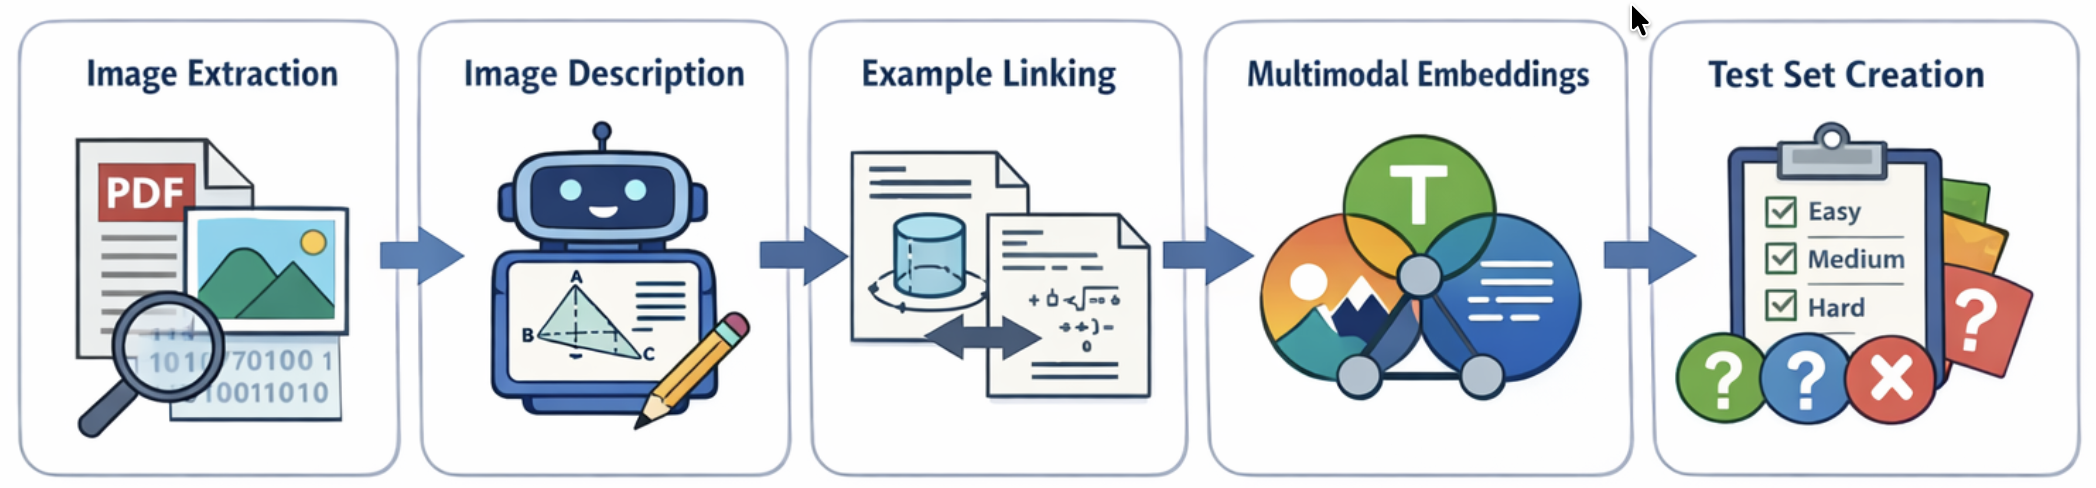
\includegraphics[width=\textwidth]{datapreprocessing.png}
    \caption{Multimodal data preprocessing pipeline consisting of image extraction, description, linking, embedding, and test set creation.}
    \label{fig:data-preprocessing}
\end{figure*}

\textbf{Stage 1 -- Image Extraction:} Using PyMuPDF, all embedded images are extracted together with metadata such as page number, position, and dimensions.

\textbf{Stage 2 -- Image Description via GPT-4V:} Each extracted image is processed with a structured prompt to generate descriptions of diagram type, labels, measurements, and mathematical concepts.

\textbf{Stage 3 -- Image-Example Linking:} Diagrams are associated with relevant worked examples using page proximity and semantic similarity.

\textbf{Stage 4 -- Multimodal Embeddings:} Joint representations are created by combining text embeddings from Sentence-BERT (768d), image embeddings from CLIP (512d), and description embeddings (768d), producing 2048-dimensional multimodal vectors indexed in ChromaDB.

\textbf{Stage 5 -- Test Set Creation:} A test set of 100 questions is created using stratified sampling, including 33 easy, 34 medium, and 33 hard questions, as well as 40 computational, 35 conceptual, and 25 proof-based questions. Each question is additionally labeled with \texttt{visual\_required}: true/false.

\subsection{System Architecture}

The proposed system follows a Retrieval-Augmented Generation (RAG) architecture consisting of four main components designed to support multimodal input processing, adaptive retrieval, and structured solution generation.


\begin{figure}[t]
    \centering
    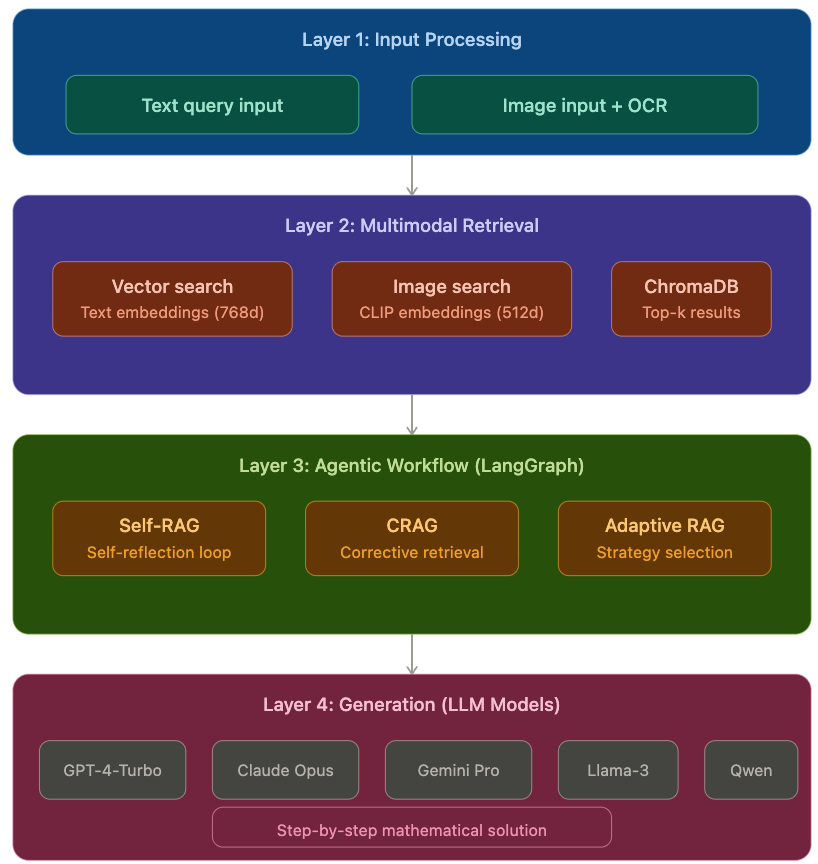
\includegraphics[width=\columnwidth]{full_architecture_diagram.png}
    \caption{Overall system architecture of the proposed multimodal RAG-based math tutoring system.}
    \label{fig:architecture}
\end{figure}

\textbf{(1) Input Processing Layer:}  
This layer handles both text-based and image-based queries. Text queries are processed directly, while image queries are first converted into textual representations using Optical Character Recognition (OCR). This enables a unified input format for downstream retrieval and reasoning.

\textbf{(2) Multimodal Retrieval Layer:}  
This layer performs joint text-image retrieval over the vector database using ChromaDB. It retrieves the top-$k$ relevant worked examples along with their associated diagrams by leveraging multimodal embeddings. This allows the system to incorporate both textual context and visual information into the reasoning process.

\textbf{(3) Agentic Workflow Layer:}  
This layer implements adaptive reasoning using LangGraph-based state machines. It supports multiple agentic workflows, including Self-RAG for iterative self-correction, CRAG for retrieval refinement, and Adaptive RAG for dynamic strategy selection. These workflows enable the system to evaluate intermediate outputs and improve solution quality through iterative reasoning.

\textbf{(4) Generation Layer:}  
This layer generates step-by-step mathematical solutions using multiple large language models. The models used in this study include GPT-4-Turbo, GPT-3.5-Turbo, Claude Opus 4.6, Gemini 1.5 Pro, and Qwen2-Math-7B. Each model is evaluated under both baseline and RAG configurations to compare general-purpose and specialized mathematical reasoning capabilities.

\section{Experiments}

We design a set of experiments to systematically evaluate the effectiveness of Retrieval-Augmented Generation (RAG), multimodal learning, and agentic workflows for curriculum-aligned mathematical problem solving. The experiments are organized into three groups: (1) baseline evaluation, (2) multimodal RAG, and (3) agentic workflow evaluation.

\subsection{Baseline LLM vs RAG}

This experiment evaluates whether Retrieval-Augmented Generation (RAG) improves mathematical problem-solving compared to baseline large language models. In the baseline setting, models generate responses using only internal knowledge, whereas in the RAG setting, models are provided with retrieved context from the Grade 10 mathematics textbook.

As shown in Table~\ref{tab:e1}, we compare multiple models under baseline and RAG settings.

\begin{table}[t]
\centering
\scriptsize
\begin{tabular}{llccc}
\toprule
Model & Setting & BLEU & ROUGE-L & BERT \\
\midrule
GPT-4-Turbo & Baseline & - & - & - \\
GPT-4-Turbo & RAG & - & - & - \\
GPT-3.5-Turbo & Baseline & - & - & - \\
GPT-3.5-Turbo & RAG & - & - & - \\
Claude Opus 4.6 & Baseline & - & - & - \\
Claude Opus 4.6 & RAG & - & - & - \\
Qwen2-Math-7B & Baseline & - & - & - \\
Qwen2-Math-7B & RAG & - & - & - \\
Gemini 1.5 Pro & Baseline & - & - & - \\
Gemini 1.5 Pro & RAG & - & - & - \\
\bottomrule
\end{tabular}
\caption{Baseline LLM vs RAG comparison.}
\label{tab:e1}
\end{table}

\subsection{Retrieval Strategy Comparison}

This experiment evaluates the impact of retrieval strategies on RAG performance. We compare vector-based retrieval with hybrid retrieval combining semantic and keyword-based matching.

\subsection{Prompt Style Comparison}

This experiment investigates how prompt design affects the quality of generated solutions. We compare general, step-by-step, and exam-oriented prompts.

\subsection{Multimodal RAG Experiments}

This experiment evaluates the impact of incorporating visual diagram information into the RAG pipeline. We compare text-only retrieval, text with image descriptions, and vision-language models.

As shown in Table~\ref{tab:e4}, we evaluate different multimodal configurations.

\begin{table}[t]
\centering
\scriptsize
\begin{tabular}{llcccc}
\toprule
Model & Modality & BLEU & ROUGE-L & BERT & Time \\
\midrule
GPT-4-Turbo & Text-only & - & - & - & - \\
GPT-4-Turbo & Text+Desc & - & - & - & - \\
GPT-4V & Text+Image & - & - & - & - \\
Claude Opus & Text+Image & - & - & - & - \\
Gemini Vision & Text+Image & - & - & - & - \\
Qwen2-Math & Text-only & - & - & - & - \\
\bottomrule
\end{tabular}
\caption{Multimodal RAG comparison.}
\label{tab:e4}
\end{table}

\subsection{Agentic RAG Experiments}

This experiment evaluates agentic RAG workflows such as Self-RAG and CRAG. These approaches introduce reflection and retrieval correction to improve solution quality.

As shown in Table~\ref{tab:e5}, we compare different agentic architectures.

\begin{table}[t]
\centering
\scriptsize
\begin{tabular}{llcccc}
\toprule
Model & Workflow & BLEU & ROUGE-L & BERT & Time \\
\midrule
GPT-4-Turbo & Baseline & - & - & - & - \\
GPT-4-Turbo & Self-RAG & - & - & - & - \\
Claude Opus & Self-RAG & - & - & - & - \\
GPT-4-Turbo & CRAG & - & - & - & - \\
Claude Opus & CRAG & - & - & - & - \\
\bottomrule
\end{tabular}
\caption{Agentic RAG comparison.}
\label{tab:e5}
\end{table}

\section{Expected Findings}

We expect that incorporating Retrieval-Augmented Generation (RAG) will significantly improve the correctness and structure of mathematical solutions compared to baseline language models, due to the inclusion of curriculum-aligned context.

For retrieval strategies, we anticipate that hybrid approaches combining semantic and keyword-based retrieval will provide more relevant context than purely vector-based methods, leading to improved generation quality.

In the multimodal setting, we expect that incorporating visual diagram information will improve performance on geometry and visually grounded problems. However, this improvement may come with increased computational cost and latency. We also expect that multimodal approaches will have limited impact on non-visual problem types such as algebra and arithmetic.

For agentic workflows, we hypothesize that Self-RAG and CRAG will improve correctness by enabling iterative refinement and retrieval correction. These approaches are expected to reduce errors caused by irrelevant context, although they may introduce additional latency due to multiple reasoning steps.

\bibliographystyle{acl_natbib}
\begin{thebibliography}{13}

\bibitem[Asai et~al.(2023)]{asai2023self}
Akari Asai, Zeqiu Wu, Yizhong Wang, Avirup Sil, and Hannaneh Hajishirzi.
\newblock 2023.
\newblock Self-RAG: Learning to Retrieve, Generate, and Critique through Self-Reflection.
\newblock \textit{arXiv preprint arXiv:2310.11511}.

\bibitem[Bubeck et~al.(2023)]{bubeck2023sparks}
Sébastien Bubeck, Varun Chandrasekaran, Ronen Eldan, Johannes Gehrke, Eric Horvitz, Ece Kamar, Peter Lee, Yin Tat Lee, Yuanzhi Li, Scott Lundberg, et~al.
\newblock 2023.
\newblock Sparks of Artificial General Intelligence: Early experiments with GPT-4.
\newblock \textit{arXiv preprint arXiv:2303.12712}.

\bibitem[Cobbe et~al.(2021)]{cobbe2021training}
Karl Cobbe, Vineet Kosaraju, Mohammad Bavarian, Mark Chen, Heewoo Jun, Lukasz Kaiser, Matthias Plappert, Jerry Tworek, Jacob Hilton, Reiichiro Nakano, et~al.
\newblock 2021.
\newblock Training Verifiers to Solve Math Word Problems.
\newblock \textit{arXiv preprint arXiv:2110.14168}.

\bibitem[Izacard and Grave(2021)]{izacard2021leveraging}
Gautier Izacard and Edouard Grave.
\newblock 2021.
\newblock Leveraging Passage Retrieval with Generative Models for Open Domain Question Answering.
\newblock In \textit{Proceedings of EACL}, pages 874--880.

\bibitem[Karpukhin et~al.(2020)]{karpukhin2020dense}
Vladimir Karpukhin, Barlas Oğuz, Sewon Min, Patrick Lewis, Ledell Wu, Sergey Edunov, Danqi Chen, and Wen-tau Yih.
\newblock 2020.
\newblock Dense Passage Retrieval for Open-Domain Question Answering.
\newblock In \textit{Proceedings of EMNLP}, pages 6769--6781.

\bibitem[Lewis et~al.(2020)]{lewis2020retrieval}
Patrick Lewis, Ethan Perez, Aleksandra Piktus, Fabio Petroni, Vladimir Karpukhin, Naman Goyal, Heinrich Küttler, Mike Lewis, Wen-tau Yih, Tim Rocktäschel, et~al.
\newblock 2020.
\newblock Retrieval-Augmented Generation for Knowledge-Intensive NLP Tasks.
\newblock In \textit{Proceedings of NeurIPS}, volume~33, pages 9459--9474.

\bibitem[OpenAI(2023)]{openai2023gpt4}
OpenAI.
\newblock 2023.
\newblock GPT-4 Technical Report.
\newblock \textit{arXiv preprint arXiv:2303.08774}.

\bibitem[Radford et~al.(2021)]{radford2021learning}
Alec Radford, Jong Wook Kim, Chris Hallacy, Aditya Ramesh, Gabriel Goh, Sandhini Agarwal, Girish Sastry, Amanda Askell, Pamela Mishkin, Jack Clark, et~al.
\newblock 2021.
\newblock Learning Transferable Visual Models From Natural Language Supervision.
\newblock In \textit{Proceedings of ICML}, pages 8748--8763.

\bibitem[Smith(2007)]{smith2007overview}
Ray Smith.
\newblock 2007.
\newblock An Overview of the Tesseract OCR Engine.
\newblock In \textit{Proceedings of ICDAR}, volume~2, pages 629--633.

\bibitem[Wei et~al.(2022)]{wei2022chain}
Jason Wei, Xuezhi Wang, Dale Schuurmans, Maarten Bosma, Brian Ichter, Fei Xia, Ed Chi, Quoc Le, and Denny Zhou.
\newblock 2022.
\newblock Chain-of-Thought Prompting Elicits Reasoning in Large Language Models.
\newblock In \textit{Proceedings of NeurIPS}, volume~35, pages 24824--24837.

\bibitem[Yan et~al.(2024)]{yan2024corrective}
Shi-Qi Yan, Jia-Chen Gu, Yun Zhu, and Zhen-Hua Ling.
\newblock 2024.
\newblock Corrective Retrieval Augmented Generation.
\newblock \textit{arXiv preprint arXiv:2401.15884}.

\bibitem[Yang et~al.(2024)]{yang2024qwen2}
An Yang, Baosong Yang, Binyuan Hui, Bo Zheng, Bowen Yu, et~al.
\newblock 2024.
\newblock Qwen2-Math Technical Report.
\newblock \textit{arXiv preprint arXiv:2409.12122}.

\bibitem[Yao et~al.(2023)]{yao2023react}
Shunyu Yao, Jeffrey Zhao, Dian Yu, Nan Du, Izhak Shafran, Karthik Narasimhan, and Yuan Cao.
\newblock 2023.
\newblock ReAct: Synergizing Reasoning and Acting in Language Models.
\newblock In \textit{Proceedings of ICLR}.

\end{thebibliography}

\end{document}